% Preprints.org submission source.
% Based on the official 2026 Preprints.org/MDPI LaTeX template supplied by the author.
\documentclass[preprints,article,submit,oneauthor]{Definitions/mdpi}

\firstpage{1}
\makeatletter
\setcounter{page}{\@firstpage}
\makeatother
\pubvolume{1}
\issuenum{1}
\articlenumber{0}
\pubyear{2026}
\copyrightyear{2026}
\datereceived{}
\daterevised{}
\dateaccepted{}
\datepublished{}

\Title{Pressure-Volume Loop Shape as a Fatigue Health Indicator for Pressure-Only Proprioception in Shared-Manifold Soft Grippers: A Simulation Study}

\Author{Mergen Ulziibayar $^{1,*}$}
\AuthorNames{Mergen Ulziibayar}

\address{%
$^{1}$ \quad Department of Mechanical and Aerospace Engineering, NYU Tandon School of Engineering, New York University, Brooklyn, NY 11201, USA; \texttt{u.mergen@nyu.edu}}

\corres{Correspondence: \texttt{u.mergen@nyu.edu}}

\abstract{Soft pneumatic grippers can lose pressure-only proprioceptive accuracy as elastomer compliance changes with cyclic fatigue, while shared-manifold architectures introduce pressure cross-talk. This simulation study evaluates whether pressure-volume (P-V) loop area can indicate fatigue-driven pose-estimation drift and trigger recalibration. A reproducible pipeline combines a standard-linear-solid pneumatic plant, a canonical fatigue law, piecewise-constant-curvature kinematics, a seeded sensor model, and shared- versus isolated-supply dynamics. The dataset contains 2,000 synthetic traces from 20 simulated actuators, partitioned by actuator identity. Shared-manifold cross-talk was measurable but second-order; a lagged-input corrector produced approximately 0\% improvement over a static ridge estimator. P-V loop-area growth correlated with fixed-calibration pose error on held-out actuators ($r=0.885$, 95\% CI [0.835, 0.958]). The deployed threshold did not provide positive temporal lead (median $-0.123$ normalized life), although lower thresholds traded additional recalibrations for earlier triggering. P-V-triggered recalibration met the 0.159 mm accuracy budget with 60\% fewer recalibrations than always-on adaptation, whereas a cycle-count schedule failed on held-out actuators. These results support P-V loop area as a simulation-derived health indicator, not a validated failure predictor. Hardware experiments are required to test device-to-device transfer.}

\keyword{soft robotics; pneumatic actuators; fatigue monitoring; pressure-volume hysteresis; proprioception; recalibration; simulation}

\begin{document}

\section{Introduction}

Soft pneumatic grippers enable safe, compliant interaction, but their deployment is limited by two monitoring problems. First, silicone chambers degrade under cyclic loading, while common durability assessments emphasize cycles to failure or compare pressure-volume (P-V) behavior before and after long fatigue campaigns \citep{mosadegh2014,mosadegh2020,wong2026}. Second, pressure-only proprioception relies on signals already present in the control loop, so changes in actuator mechanics can make a previously calibrated pressure-to-pose map stale \citep{wang2020}.

Multi-finger grippers commonly share a pneumatic source to reduce valve count, mass, and onboard hardware \citep{mcdonald2021,moran2024}. In this topology, one chamber's valve command perturbs the shared supply node and therefore its neighbors. Fatigue-induced compliance drift could consequently alter both P-V loop shape and inter-chamber cross-talk. This raises a practical question: can one in-loop fluidic signal support both health monitoring and pressure-only pose estimation?

This paper evaluates that question in a transparent simulation before hardware testing. The pipeline couples a viscoelastic pneumatic plant, a canonical fatigue law, piecewise-constant-curvature (PCC) kinematics, a reproducible sensor model, and shared- versus isolated-supply dynamics. The analysis tests three propositions: whether a dynamic corrector benefits from shared-manifold history, whether observable P-V loop area tracks pose-estimation degradation, and whether a P-V-triggered policy can reduce recalibration effort without exceeding a stated accuracy budget.

The study reports synthetic modeling results, not measurements from physical actuators. All simulated actuators are generated by one model family. Held-out evaluation therefore tests robustness to parameter variation within that generator and does not establish transfer to manufactured devices.

\section{Related Work and Prior-Art Boundary}

\subsection{P-V hysteresis and fatigue monitoring}

P-V hysteresis is established as a before-and-after durability diagnostic for pneumatic networks \citep{mosadegh2014,mosadegh2020}, and fatigue-related shifts have been reported for PneuNet actuators \citep{libby2023}. Elastomer-fatigue mechanics further distinguish irreversible damage from Mullins softening and rest-dependent recovery \citep{mars2002,lavazza2023,liao2021}. The present study therefore does not claim the first use of P-V behavior for fatigue. Its narrower contribution is a cycle-resolved, operational loop-area health signal connected to a recalibration policy.

Hysteresis-loop area has also been used as a damage-sensitive quantity outside soft robotics \citep{haghshenas2021,guo2021,galanopoulos2023}. General prognostics frameworks emphasize that a useful health indicator must be evaluated for monotonicity, trendability, and operational decision value rather than correlation alone \citep{scheffer2009,lei2018}. Accordingly, this study reports both correlation and trigger timing.

\subsection{Pressure-only proprioception and drift compensation}

Pressure-only and fluidic self-sensing methods infer configuration, displacement, force, or contact without adding external strain sensors \citep{wang2020,wang2023,wang2025,joshi2023,zou2024,preechayasomboon2021}. These studies generally assume clean per-actuator inputs. Lindenroth et al. \citep{lindenroth2023} addressed sensing in coupled parallel chambers but did not connect shared-manifold cross-talk to fatigue-driven proprioception drift.

Recurrent and reservoir-based models can compensate pneumatic hysteresis \citep{jaeger2004,youssef2022,shen2025}. Online adaptation has also been used for time-varying soft sensors \citep{thuruthel2022,kushawaha2025}. The contrast evaluated here is event-driven recalibration using a measured P-V health state rather than continuous adaptation or a cycle-count clock.

\subsection{Shared-manifold modeling and evaluation}

Lumped resistance-compliance models provide a compact representation of pneumatic circuit dynamics \citep{stanley2021}. Shared-source valve architectures are relevant to onboard multi-degree-of-freedom systems \citep{mcdonald2021,moran2024}. This study uses that modeling framework to separate static behavior from actuation-band cross-talk. Pose is defined through PCC kinematics \citep{webster2010}, and the train-test split follows soft-proprioception evaluation guidance by separating actuator identities rather than traces \citep{zhang2023}.

\section{Materials and Methods}

\subsection{Study design and reproducibility}

The pipeline is implemented in Python in the public project repository. All randomness is seeded, each stage is covered by automated checks, and dataset integrity is pinned by a SHA-256 manifest. The analysis state is identified by the repository tag \texttt{preprint-v1.3}.

\subsection{Viscoelastic pneumatic plant}

Chamber walls are represented by a standard linear solid in the pressure-volume analog: a spring $k_1$ in parallel with a Maxwell arm having spring $k_2$ and relaxation time $\tau$. The resulting rate-dependent P-V loop has closed-form dissipated energy
\begin{equation}
E_{\mathrm{loss}}(\omega)=\pi k_2 A^2\frac{\omega\tau}{1+(\omega\tau)^2},
\end{equation}
which is used as a numerical validation check. In the quasi-static limit, the plant reduces to the linear model used for the initial cross-talk gate.

\subsection{Canonical fatigue model}

The deterministic life law combines a 30\% permanent Mullins floor, a 24 h recovery time constant, irreversible compliance drift, curvature-acceleration onset at 70\% of normalized life, and late leak growth to 20 times the initial conductance. Degradation enters the plant through a rising compliance multiplier and loss multiplier. Leakage is observed with a separate closed-valve pressure-decay probe; it is not inferred from the imposed-volume P-V loop.

\subsection{P-V features and health signal}

Causal loop features are normalized against the young state after accounting for reversible Mullins recovery. The deployed health signal is observable fractional P-V loop-area growth, not ground-truth compliance. The feature pipeline was checked across a 144-condition synthetic identifiability grid before being applied to the downstream studies.

\subsection{Fatigue-coupled kinematics}

Realized chamber pressure maps to bending curvature through
\begin{equation}
\kappa=\kappa_{\mathrm{gain}}\,C(\ell)\max(P-P_0,0),
\end{equation}
where $C(\ell)$ is the life-dependent compliance multiplier. Curvature maps to tip pose using the PCC convention \citep{webster2010}. Forward and inverse mappings are checked by round-trip tests, and noise-free pose recovery is exact to numerical precision.

\subsection{Sensor model}

The measurement model applies seeded Gaussian noise, quantization, decimation, and a synthetic contact observation. Independent random sub-streams for each channel make the corruption reproducible and invariant to channel ordering.

\subsection{Shared and isolated supply dynamics}

A time-domain integrator drives one focal chamber and two neighbors. In the shared topology, all chambers draw from one supply node; in the isolated topology, each chamber has a regulated node and the state blocks are decoupled. Multisine excitation spans the 1-5 Hz actuation band. Gate checks require isolated coupling below $10^{-6}$, measurable shared coupling above $10^{-4}$, compliance-independent direct-current gain, and fatigue-dependent actuation-band gain.

\subsection{Synthetic dataset and split}

The dataset contains
\begin{equation}
20\ \mathrm{actuators}\times5\ \mathrm{life\ stages}\times2\ \mathrm{topologies}\times2\ \mathrm{contact\ states}\times5\ \mathrm{repetitions}=2{,}000\ \mathrm{traces}.
\end{equation}
Each trace contains 240 time samples. Geometry, wall stiffness, and rupture life are drawn deterministically for each simulated actuator. Fourteen actuator identities are used for training and six are held out. No actuator contributes traces to both partitions.

\subsection{Pressure-only correctors}

The prediction target is focal bending curvature and, through the PCC map, tip position. Inputs are shared-manifold pressure and all chamber commands. A static ridge estimator is compared with the same ridge model applied to lagged inputs, forming an exogenous ARX/FIR corrector. Output feedback is excluded because pose is the estimation target rather than an online measurement.

\subsection{Recalibration policies and statistical analysis}

Four policies are evaluated from a common young-state calibration: fixed, cycle-count scheduled, P-V triggered, and always-on. The triggered policy recalibrates when loop-area growth since the last calibration exceeds $\tau$. The cycle-count policy recalibrates every $T$ cycles. Both $\tau$ and $T$ are selected on training actuators using the same rule: minimize recalibration count while satisfying the 0.159 mm accuracy budget. The selected settings are then applied unchanged to held-out actuators.

Pearson correlation between observable loop-area growth and fixed-calibration pose error is reported with a 95\% bootstrap confidence interval from 2,000 resamples. Trigger and budget-crossing times are linearly interpolated between the five simulated life stages. Error and recalibration count are reported together.

\subsection{Use of generative artificial intelligence}

OpenAI Codex (GPT-5) was used to reorganize and language-edit the manuscript and to assist with conversion to the Preprints.org LaTeX template. All reported values remain tied to frozen repository outputs and automated manuscript-number checks. The author reviewed and edited the resulting text and takes full responsibility for the content.

\section{Results}

\subsection{Validation gates}

The structural checks passed: noise-free pose recovery and forward-inverse curvature round trips reached numerical precision; isolated-supply off-diagonal coupling remained below $10^{-6}$ while shared coupling exceeded $10^{-4}$; and the direct-current versus actuation-band cross-talk properties matched the intended lumped model.

\subsection{Cross-talk was measurable but second-order}

The initial prediction was that shared-manifold history would favor the lagged-input corrector over the static ridge estimator. This prediction was not supported. Curvature RMSE was 0.244 versus 0.244 m$^{-1}$ for the shared topology and 0.295 versus 0.295 m$^{-1}$ for the isolated topology. Corresponding pose errors were approximately 0.84 versus 0.84 mm and 1.02 versus 1.02 mm. The dynamic corrector therefore produced approximately 0\% improvement under either topology. Cross-talk was present in the network dynamics but amounted to approximately 4\% of focal curvature under the default parameters.

\begin{figure}[H]
\isPreprints{\centering}{}

\includegraphics[width=0.84\textwidth]{figures/study2_fig2_static_vs_dynamic.png}
\caption{Static and lagged-input correctors evaluated on held-out actuators at old life. The expected shared-manifold advantage of the lagged model did not appear.\label{fig:correctors}}
\end{figure}

\subsection{Compliance drift dominated pose-estimation error}

A static estimator calibrated at the young state showed curvature RMSE growth from approximately 0.004 m$^{-1}$ to approximately 0.46-0.56 m$^{-1}$ at life 0.9. Shared and isolated trends were comparable. Under the simulated conditions, topology-independent compliance-scale drift therefore dominated the pressure-only proprioception error.

\begin{figure}[H]
\isPreprints{\centering}{}

\includegraphics[width=0.84\textwidth]{figures/study2_fig1_drift.png}
\caption{Curvature RMSE of the young-calibrated static estimator across normalized life. Error increased by roughly two orders of magnitude and remained comparable between supply topologies.\label{fig:drift}}
\end{figure}

\subsection{P-V loop area tracked degradation but did not lead at the deployed threshold}

On held-out actuators, fractional P-V loop-area growth correlated with fixed-calibration pose error with Pearson $r=0.885$ and 95\% CI [0.835, 0.958]. Per-actuator $r$ had median 0.957 and range [0.9570, 0.9574]. This narrow range is a generator property: young normalization makes the P-V health trajectory numerically identical across the simulated actuator draws.

At the train-selected threshold $\tau^{*}=0.05$, the trigger crossed at life 0.83, while the accuracy budget crossed earlier at median life 0.71, range 0.56-0.71. The resulting median lead was $-0.123$ normalized life, range [$-0.269$, $-0.115$], corresponding to approximately $-972$ to $-375$ cycles; all 6/6 held-out actuators had nonpositive lead. Lowering the threshold to $\tau=0.01$ shifted the median trigger to life 0.36 and produced median lead $+0.346$, range $+0.199$ to $+0.354$, with 3 recalibrations and 0.029 mm pose RMSE. At $\tau=0.02$, error remained within budget at 0.037 mm, but 1/6 held-out actuators still had nonpositive lead. At $\tau=0.005$, the policy fired at every life stage and matched always-on performance with 5 recalibrations and 0.019 mm error. The selected threshold consumed approximately 77\% of the signal's 6.5\% dynamic range.

\begin{figure}[H]
\isPreprints{\centering}{}
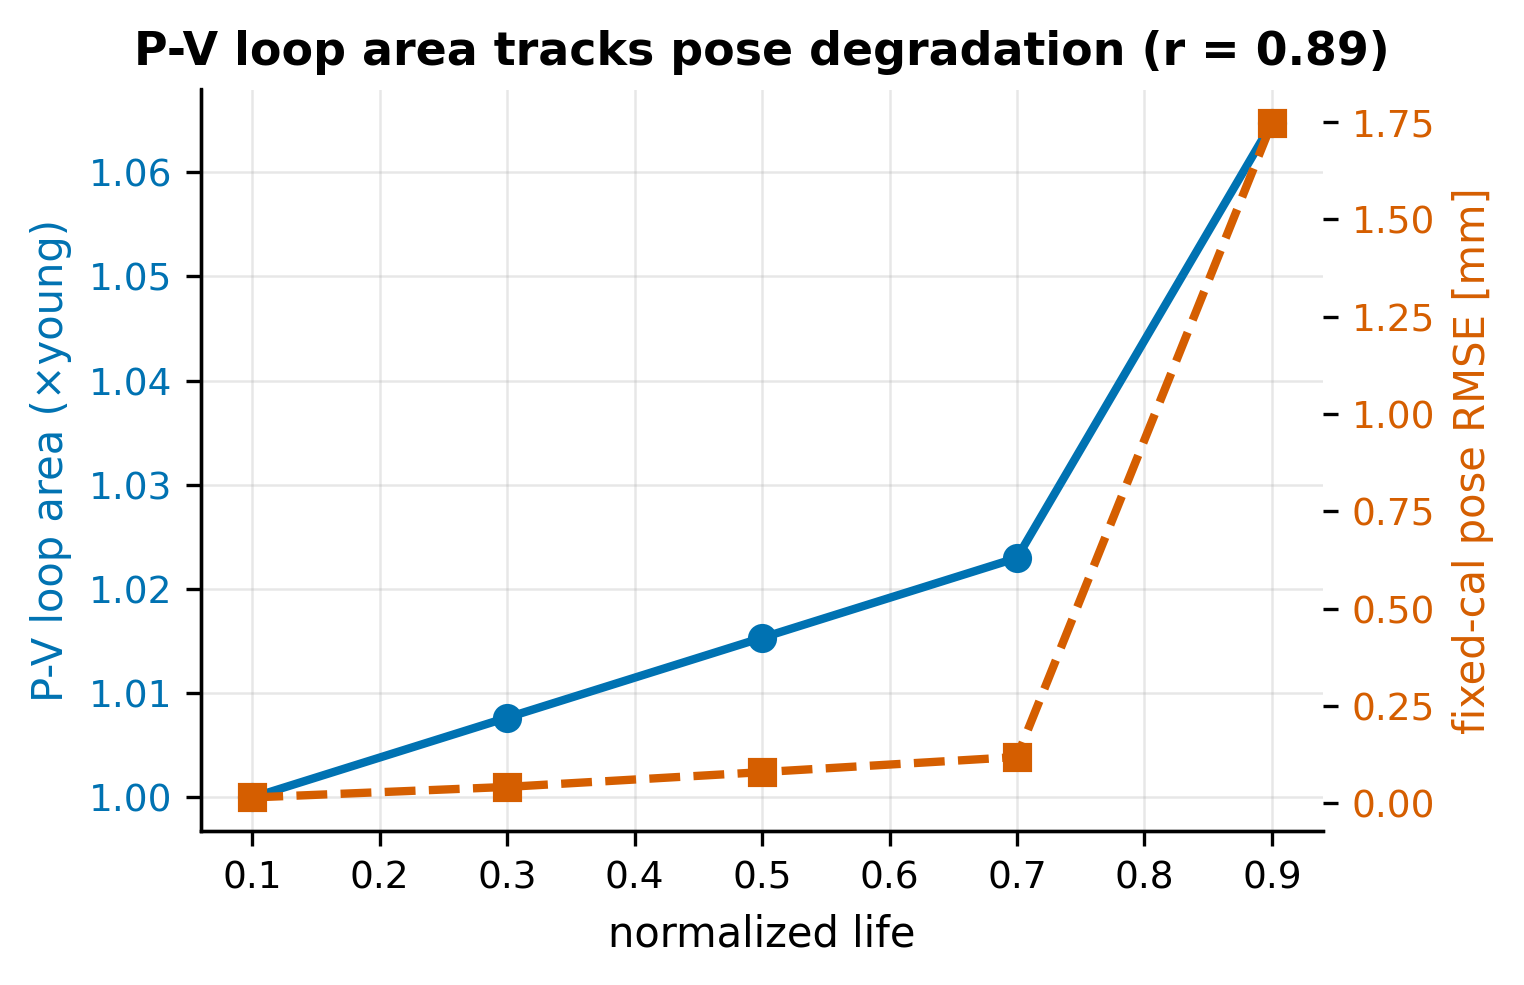
\includegraphics[width=0.84\textwidth]{figures/study3_fig3_leading_indicator.png}
\caption{Observable P-V loop-area growth and fixed-calibration pose error on held-out actuators. The selected threshold had no positive temporal lead; lower thresholds form a lead-versus-recalibration frontier.\label{fig:health}}
\end{figure}

\subsection{P-V-triggered recalibration met the accuracy budget}

Both adaptive policies were tuned on training actuators with the same rule. The selected P-V threshold was $\tau^{*}=0.05$, and the selected cycle period was $T^{*}=2{,}700$ cycles. On held-out actuators, the P-V-triggered policy met the 0.159 mm accuracy budget with 0.06 mm pose RMSE and 2 recalibrations per actuator. This is 60\% fewer recalibrations than always-on adaptation. The cycle-count policy produced 0.21 mm RMSE with 1.5 recalibrations and failed the budget after transfer.

\begin{table}[H]
\caption{Recalibration policies evaluated on held-out actuators.\label{tab:policies}}
\begin{tabularx}{\textwidth}{lCCC}
\toprule
\textbf{Policy} & \textbf{Pose RMSE} & \textbf{Recalibrations} & \textbf{Budget met} \\
\midrule
Fixed & 0.40 mm & 1 & No \\
Cycle-count, $T^{*}=2{,}700$ & 0.21 mm & 1.5 & No \\
P-V-triggered, $\tau^{*}=0.05$ & 0.06 mm & 2 & Yes \\
Always-on & 0.02 mm & 5 & Yes \\
\bottomrule
\end{tabularx}
\end{table}

\begin{figure}[H]
\isPreprints{\centering}{}
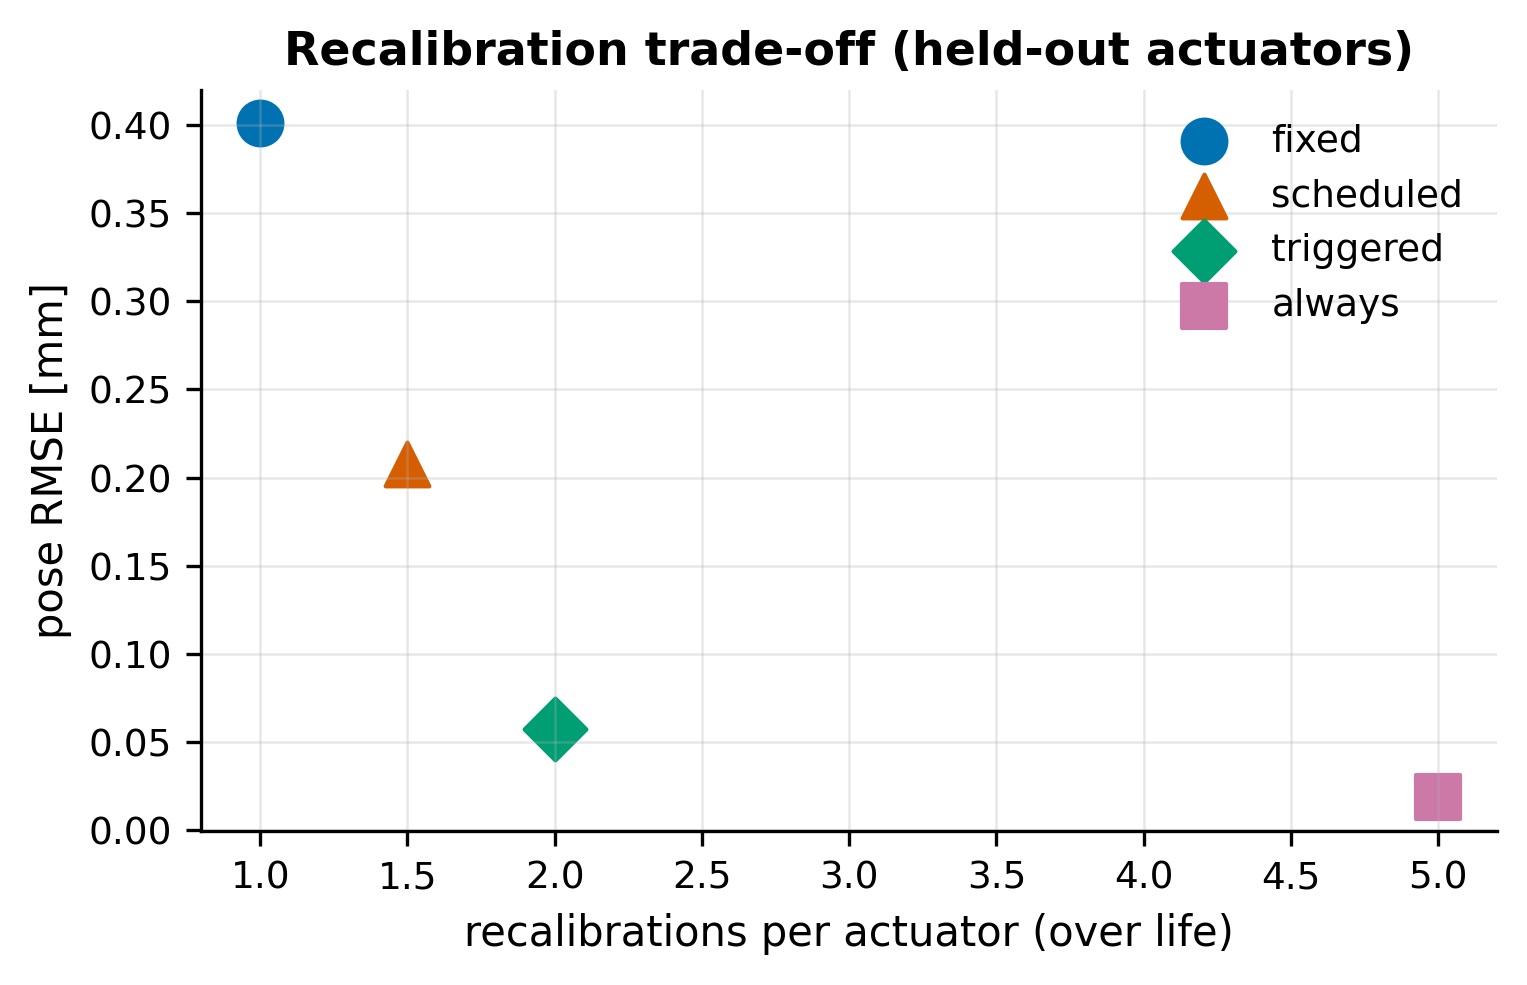
\includegraphics[width=0.84\textwidth]{figures/study3_fig4_recal_tradeoff.png}
\caption{Pose error versus recalibration count on held-out actuators. The P-V-triggered policy met the budget with fewer recalibrations than always-on adaptation, while the cycle-count schedule failed after transfer.\label{fig:tradeoff}}
\end{figure}

\subsection{Cross-talk sensitivity envelope}

At the default parameters, the neighbor-to-driven coupling ratio was 6.3\%. It reached 10\% when supply resistance was approximately $1.7\times$ softer and 20\% at approximately $4.3\times$ softer. Across a 128-fold manifold-compliance sweep from $0.25\times$ to $32\times$, coupling remained within 5.8-6.3\%. The default result was therefore not a single-point cancellation; cross-talk became first-order only with a substantially under-provisioned supply.

\begin{figure}[H]
\isPreprints{\centering}{}
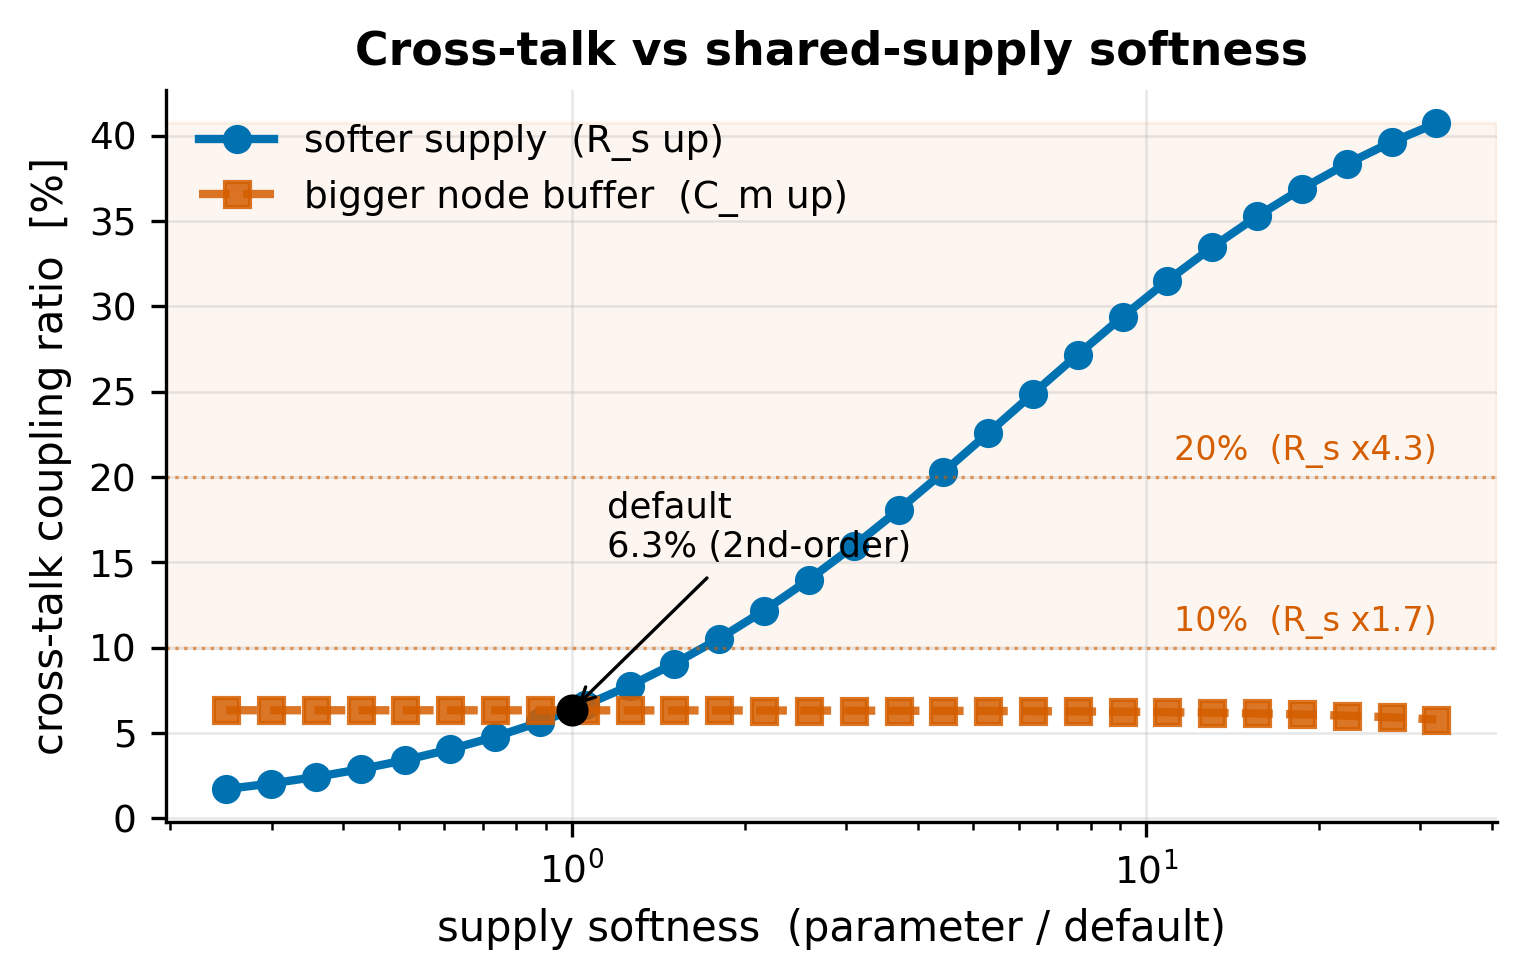
\includegraphics[width=0.84\textwidth]{figures/study4_fig_crosstalk_sensitivity.png}
\caption{Neighbor-to-driven coupling ratio versus shared-supply softness. Supply resistance was the dominant sensitivity parameter; manifold compliance produced only a narrow change around the default coupling level.\label{fig:sensitivity}}
\end{figure}

\section{Discussion}

\subsection{Interpretation}

The simulation separates two effects that were initially expected to interact strongly. Shared-manifold cross-talk was real and fatigue-dependent in the actuation band, but it remained too small to make a lagged corrector outperform a static ridge model under the tested conditions. The dominant error pathway was the life-dependent compliance scale, which altered the pressure-to-curvature map in both supply topologies.

Observable P-V loop area tracked that drift and supported a useful recalibration policy, but correlation did not guarantee warning lead. The deployed threshold fired after the accuracy budget had already been crossed. Lower thresholds recovered positive lead by accepting more recalibrations. Trigger sensitivity is therefore an operating trade-off rather than an intrinsic property of the signal.

The comparison with the cycle-count schedule isolates the value of the measured P-V state. In this generator, rupture life varies across actuators, so one global cycle interval misaligns with device state. The normalized P-V signal transfers more safely because it acts as a simulated state measurement. This result should not be generalized to physical actuators until device-to-device fatigue trajectories are measured.

\subsection{Limitations}

All results are synthetic. The 20 actuators are samples from one generator, not 20 manufactured devices, and young normalization makes the P-V health trajectory nearly identical across actuator draws. The reported confidence interval therefore quantifies variation within the simulated analysis, not population uncertainty for silicone actuators.

The fatigue law, single-segment PCC kinematics, lumped pneumatic network, sensor noise, and contact model are transparent design assumptions rather than calibrated fits. Real devices can introduce delamination, local tearing, temperature dependence, manufacturing variability, regulator dynamics, and measurement drift not represented here. Absolute pose errors also remained below 1 mm, so the practical value of triggered recalibration depends on the accuracy requirements of the application.

\subsection{Next experimental test}

The next step is a physical bench study that measures P-V loops, pose, temperature, rest history, and failure progression on multiple actuators. An initial spot check should establish whether loop-area changes remain distinguishable from Mullins recovery and sensor drift. A subsequent fatigue campaign should test whether the train-selected trigger transfers across independently manufactured devices.

\section{Conclusions}

Within one simulation generator, P-V loop area acted as a quantified health indicator of fatigue-driven pressure-only proprioception drift. The selected P-V-triggered policy met a 0.159 mm accuracy budget with 60\% fewer recalibrations than always-on adaptation, while a cycle-count policy failed after transfer to held-out simulated actuators. Shared-manifold cross-talk was measurable but second-order for pose under the tested parameters, and a lagged corrector did not outperform a static model. The selected trigger did not provide positive temporal lead on the five-stage grid. The evidence supports further hardware testing of P-V-based recalibration; it does not establish a validated physical failure predictor.

\supplementary{The source code, frozen result files, figures, and reproduction commands are available at \url{https://github.com/500ft/P-V-Fatigue-Manifold-Proprioception}. The simulation state analyzed in this manuscript is identified by the tag \texttt{preprint-v1.3}.}

\authorcontributions{Conceptualization, M.U.; methodology, M.U.; software, M.U.; validation, M.U.; formal analysis, M.U.; investigation, M.U.; data curation, M.U.; writing - original draft preparation, M.U.; writing - review and editing, M.U.; visualization, M.U.; project administration, M.U. The author has read and agreed to the published version of the manuscript.}

\funding{This research received no external funding.}

\institutionalreview{Not applicable. This study used simulation data and did not involve humans or animals.}

\informedconsent{Not applicable.}

\dataavailability{All simulation code, frozen result JSON files, generated figures, tests, and reproduction instructions are publicly available at \url{https://github.com/500ft/P-V-Fatigue-Manifold-Proprioception}. The analyzed state is pinned by the tag \texttt{preprint-v1.3}. The dataset can be regenerated from a fixed seed using \texttt{python -m scripts.phaseD\_dataset}; integrity is recorded in the committed SHA-256 manifest.}

\acknowledgments{No additional acknowledgments.}

\conflictsofinterest{The author declares no conflicts of interest.}

\abbreviations{Abbreviations}{%
The following abbreviations are used in this manuscript:\\
\noindent
\begin{tabular}{@{}ll}
ARX/FIR & Autoregressive with exogenous inputs / finite impulse response\\
CI & Confidence interval\\
PCC & Piecewise-constant curvature\\
P-V & Pressure-volume\\
RMSE & Root-mean-square error\\
\end{tabular}
}

\reftitle{References}

\begin{thebibliography}{99}

\bibitem{mosadegh2014}
Mosadegh, B.; Polygerinos, P.; Keplinger, C.; Wennstedt, S.; Shepherd, R.F.; Gupta, U.; Shim, J.; Bertoldi, K.; Walsh, C.J.; Whitesides, G.M. Pneumatic networks for soft robotics that actuate rapidly. \emph{Adv. Funct. Mater.} \textbf{2014}, \emph{24}, 2163-2170. \href{https://doi.org/10.1002/adfm.201303288}{doi:10.1002/adfm.201303288}.

\bibitem{mosadegh2020}
Mosadegh, B.; Shepherd, R.F.; Whitesides, G.M. Low strain pneumatic networks for soft robots. U.S. Patent US10639801B2, 5 May 2020.

\bibitem{wong2026}
Wong, C.; Luo, Y.; Scharff, R.B.N. Durability of soft pneumatic actuators: A review and benchmarking protocol. \emph{Adv. Robot. Res.} \textbf{2026}, e202500172. \href{https://doi.org/10.1002/adrr.202500172}{doi:10.1002/adrr.202500172}.

\bibitem{wang2020}
Wang, L.; Wang, Z. Mechanoreception for soft robots via intuitive body cues. \emph{Soft Robot.} \textbf{2020}, \emph{7}, 198-217. \href{https://doi.org/10.1089/soro.2018.0135}{doi:10.1089/soro.2018.0135}.

\bibitem{mcdonald2021}
McDonald, K.; Ranzani, T. Hardware methods for onboard control of fluidically actuated soft robots. \emph{Front. Robot. AI} \textbf{2021}, \emph{8}, 720702. \href{https://doi.org/10.3389/frobt.2021.720702}{doi:10.3389/frobt.2021.720702}.

\bibitem{moran2024}
Moran, M.E.; et al. An electropermanent magnet valve for the onboard control of multi-DoF pneumatic soft robots. \emph{Commun. Eng.} \textbf{2024}, \emph{3}, 117. \href{https://doi.org/10.1038/s44172-024-00251-y}{doi:10.1038/s44172-024-00251-y}.

\bibitem{libby2023}
Libby, T.; et al. What happens when Pneu-Net soft robotic actuators get fatigued? In \emph{Proceedings of the 2023 International Symposium on Medical Robotics}; IEEE: 2023. \href{https://doi.org/10.1109/ISMR57123.2023.10130227}{doi:10.1109/ISMR57123.2023.10130227}.

\bibitem{mars2002}
Mars, W.V.; Fatemi, A. A literature survey on fatigue analysis approaches for rubber. \emph{Int. J. Fatigue} \textbf{2002}, \emph{24}, 949-961. \href{https://doi.org/10.1016/S0142-1123(02)00008-7}{doi:10.1016/S0142-1123(02)00008-7}.

\bibitem{lavazza2023}
Lavazza, M.; Contino, M.; Marano, C. Strain rate, temperature and deformation state effect on Ecoflex 00-50 silicone mechanical behaviour. \emph{Mech. Mater.} \textbf{2023}, \emph{178}, 104560. \href{https://doi.org/10.1016/j.mechmat.2023.104560}{doi:10.1016/j.mechmat.2023.104560}.

\bibitem{liao2021}
Liao, Z.; et al. On the stress recovery behaviour of Ecoflex silicone rubbers. \emph{Int. J. Mech. Sci.} \textbf{2021}, \emph{206}, 106624. \href{https://doi.org/10.1016/j.ijmecsci.2021.106624}{doi:10.1016/j.ijmecsci.2021.106624}.

\bibitem{haghshenas2021}
Haghshenas, A.; Jang, S.; Khonsari, M.M. On the intrinsic dissipation and fracture fatigue entropy of metals. \emph{Mech. Mater.} \textbf{2021}, \emph{155}, 103734. \href{https://doi.org/10.1016/j.mechmat.2020.103734}{doi:10.1016/j.mechmat.2020.103734}.

\bibitem{guo2021}
Guo, Y.; Ma, C.; Dong, X.; Liang, Y.; Hu, B. A novel health indicator based on hysteresis loop for health prediction of flight control systems. \emph{Measurement} \textbf{2021}, \emph{186}, 110076. \href{https://doi.org/10.1016/j.measurement.2021.110076}{doi:10.1016/j.measurement.2021.110076}.

\bibitem{galanopoulos2023}
Galanopoulos, G.; et al. Acoustic emission-based remaining useful life prognosis of aeronautical structures. \emph{Eng. Struct.} \textbf{2023}, \emph{290}, 116391. \href{https://doi.org/10.1016/j.engstruct.2023.116391}{doi:10.1016/j.engstruct.2023.116391}.

\bibitem{scheffer2009}
Scheffer, M.; et al. Early-warning signals for critical transitions. \emph{Nature} \textbf{2009}, \emph{461}, 53-59. \href{https://doi.org/10.1038/nature08227}{doi:10.1038/nature08227}.

\bibitem{lei2018}
Lei, Y.; Li, N.; Guo, L.; Li, N.; Yan, T.; Lin, J. Machinery health prognostics: A systematic review from data acquisition to RUL prediction. \emph{Mech. Syst. Signal Process.} \textbf{2018}, \emph{104}, 799-834. \href{https://doi.org/10.1016/j.ymssp.2017.11.016}{doi:10.1016/j.ymssp.2017.11.016}.

\bibitem{wang2023}
Wang, L.; et al. Soft robot proprioception using unified soft body encoding and recurrent neural networks. \emph{Soft Robot.} \textbf{2023}, \emph{10}, 825-837. \href{https://doi.org/10.1089/soro.2021.0056}{doi:10.1089/soro.2021.0056}.

\bibitem{wang2025}
Wang, J.; et al. Proprioceptive and exteroceptive information perception in a fabric soft robotic arm via physical reservoir computing. \emph{Adv. Intell. Syst.} \textbf{2025}, \emph{7}, 2400534. \href{https://doi.org/10.1002/aisy.202400534}{doi:10.1002/aisy.202400534}.

\bibitem{joshi2023}
Joshi, S.; Paik, J. Sensorless force and displacement estimation in soft actuators. \emph{Soft Matter} \textbf{2023}, \emph{19}. \href{https://doi.org/10.1039/D2SM01197B}{doi:10.1039/D2SM01197B}.

\bibitem{zou2024}
Zou, J.; et al. A retrofit sensing strategy for soft fluidic robots. \emph{Nat. Commun.} \textbf{2024}, \emph{15}, 539. \href{https://doi.org/10.1038/s41467-023-44517-z}{doi:10.1038/s41467-023-44517-z}.

\bibitem{preechayasomboon2021}
Preechayasomboon, P.; Rombokas, E. Sensuator: A hybrid sensor-actuator approach to soft robotic proprioception using recurrent neural networks. \emph{Actuators} \textbf{2021}, \emph{10}, 30. \href{https://doi.org/10.3390/act10020030}{doi:10.3390/act10020030}.

\bibitem{lindenroth2023}
Lindenroth, L.; Stoyanov, D.; Rhode, K.; Liu, H. Toward intrinsic force sensing and control in parallel soft robots. \emph{IEEE/ASME Trans. Mechatron.} \textbf{2023}, \emph{28}, 80-91. \href{https://doi.org/10.1109/TMECH.2022.3210065}{doi:10.1109/TMECH.2022.3210065}.

\bibitem{jaeger2004}
Jaeger, H.; Haas, H. Harnessing nonlinearity: Predicting chaotic systems and saving energy in wireless communication. \emph{Science} \textbf{2004}, \emph{304}, 78-80. \href{https://doi.org/10.1126/science.1091277}{doi:10.1126/science.1091277}.

\bibitem{youssef2022}
Youssef, I.; et al. Modeling of soft pneumatic actuators using echo state networks. \emph{Micromachines} \textbf{2022}, \emph{13}, 216. \href{https://doi.org/10.3390/mi13020216}{doi:10.3390/mi13020216}.

\bibitem{shen2025}
Shen, Z.; Miyazaki, R.; Kawashima, K. Feedforward hysteresis compensation by pneumatic physical reservoir computing. \emph{IEEE Robot. Autom. Lett.} \textbf{2025}; arXiv:2409.06961.

\bibitem{thuruthel2022}
Thuruthel, T.G.; Gardner, M.; Iida, F. Closing the control loop with time-variant embedded soft sensors and recurrent neural networks. \emph{Soft Robot.} \textbf{2022}, \emph{9}, 1167-1176. \href{https://doi.org/10.1089/soro.2021.0012}{doi:10.1089/soro.2021.0012}.

\bibitem{kushawaha2025}
Kushawaha, A.; et al. Adaptive drift compensation for soft sensorized finger using continual learning. \textbf{2025}; arXiv:2503.16540.

\bibitem{stanley2021}
Stanley, A.A.; Amini, A.; Glick, P.; Usevitch, N.; Menguec, Y.; Keller, S. Lumped-parameter response time models for pneumatic circuit dynamics. \emph{J. Dyn. Syst. Meas. Control} \textbf{2021}, \emph{143}, 051001. \href{https://doi.org/10.1115/1.4049009}{doi:10.1115/1.4049009}.

\bibitem{webster2010}
Webster, R.J.; Jones, B.A. Design and kinematic modeling of constant curvature continuum robots: A review. \emph{Int. J. Robot. Res.} \textbf{2010}, \emph{29}, 1661-1683. \href{https://doi.org/10.1177/0278364910368147}{doi:10.1177/0278364910368147}.

\bibitem{zhang2023}
Zhang, Y.; Wang, H.; Truby, R.L.; Chin, L.; Rus, D. Machine learning best practices for soft robot proprioception. In \emph{Proceedings of the 2023 IEEE/RSJ International Conference on Intelligent Robots and Systems}; IEEE: 2023; pp. 2564-2571. \href{https://doi.org/10.1109/IROS55552.2023.10342379}{doi:10.1109/IROS55552.2023.10342379}.

\end{thebibliography}

\PublishersNote{}
\end{document}
